%
\hsection{The Feasibility of the Solutions}%
\label{sec:solutionSpace:feasibility}%
%
For many optimization problems, we can pick any element~\solspel\ from the solution space~\solutionSpace\ and return it as output of an optimization algorithm.
For many \emph{other} optimization problems, some elements of~\solutionSpace\ are not permissible for different reasons.
We we call these reasons \emph{constraints}.%
%
\hsection{Definitions}%
%
\begin{definition}[Constraint]%
\label{def:constraint}%
A \emph{constraint} is a rule imposed on the solution space~\solutionSpace\ which can either be fulfilled or violated by a candidate solution~$\solspel\in\solutionSpace$.%
\end{definition}%
%
\begin{definition}[Feasibility]%
\label{def:feasibility}%
A candidate solution~$\solspel\in\solutionSpace$ is \emph{feasible} if and only if it fulfills all constraints.%
\end{definition}%
%
\begin{definition}[Infeasibility]%
\label{def:infeasibility}%
A candidate solution~$\solspel\in\solutionSpace$ is \emph{infeasible} if it is \emph{not feasible}, i.e., if it violates at least one constraint.%
\end{definition}%
%
\endhsection%
%
\hsection{A Programmer's Perspective}%
%
There is not much to discuss here from a programmer's perspective because there are many different ways to deal with constraints.
In our \moptipy\ \codeil{Space} API illustrated in \autoref{lst:Space}, we provide the method \codeil{validate}.
The programmer can implement this method to check whether a solution is feasible or not.
If not, the method is supposed to throw a \codeil{ValueError} if it is not.%
%
\endhsection%
%
\hsection{Example: Job Shop Scheduling}%
%
In order to be a feasible solution for a \gls{JSSP} instance, a Gantt chart must indeed fulfill a couple of \emph{constraints}:%
%
\begin{enumerate}
%
\item All operations of all jobs must be assigned to their respective machines and properly be completed.%
%
\item Only the jobs and machines specified by the problem instance must occur in the chart.%
%
\item An operation must be assigned a time window on its corresponding machine which is exactly as long as the operation needs on that machine.%
%
\item The operations of one job cannot intersect or overlap. %
The next operation of one job can only begin after the previous operation of the job has been completed.%
%
\item Each machine can only carry out one operation at a time.%
%
\item Once a machine begins to process an operation, it cannot stop until the operation is complete, i.e., no preemption is possible%
%
\item The precedence constraints of the operations must be honored. %
In other words, if the instance says that operation~1 of job~1 should take place before operation~2 of job~1, then this must also be the case in the Gantt chart.%
%
\end{enumerate}%
%
While the first six \emph{constraints} are rather trivial, the latter one proofs problematic.
Imagine a \gls{JSSP} with $\jsspJobs=2$~jobs and $\jsspMachines=2$~machines.
There are $(2!)^2=(1*2)^2=4$~possible Gantt charts.
Assume that the first job needs to first be processed by machine~0 and then by machine~1, while the second job first needs to go to machine~1 and then to machine~0.
A Gantt chart which assigns the first job to be the first on machine~1 and the second job first to be the first on machine~$0$ cannot be executed in practice, i.e., is \emph{infeasible}, as such an assignment does not honor the precedence constraints of the jobs.
Instead, it contains a deadlock.

\begin{figure}%
\centering%
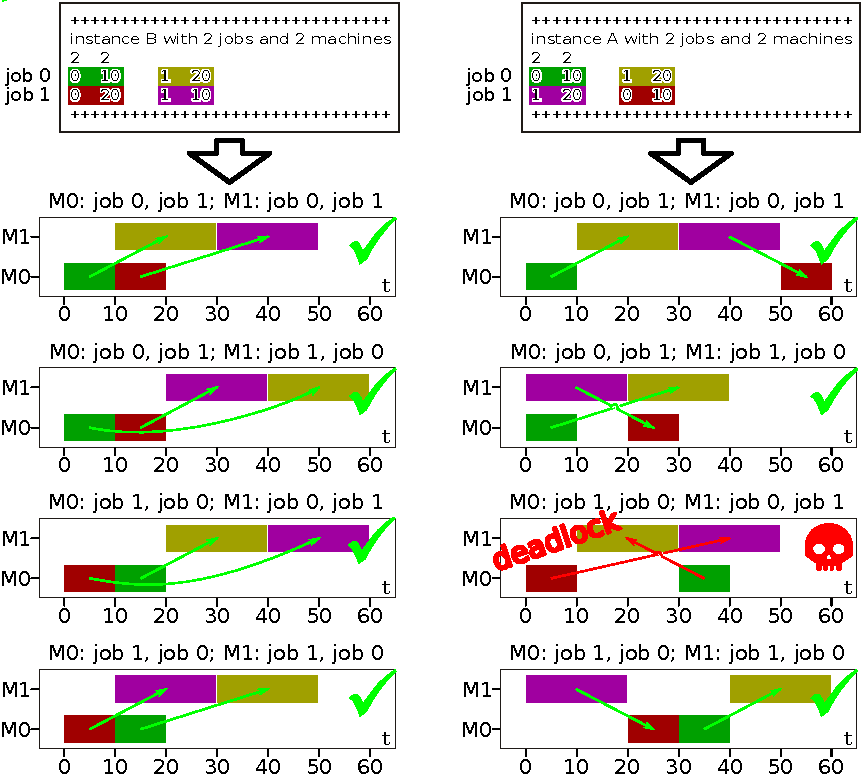
\includegraphics[width=0.85\linewidth]{\currentDir/jssp_feasible_gantt.pdf}%
\caption{Two different JSSP instances with $\jsspMachines=2$~machines and $\jsspJobs=2$~jobs.%
The left one has four feasible corresponding Gantt charts.
The right one has only three feasible solutions and one infeasible one.}%
\label{fig:jssp_feasible_gantt}%
\end{figure}%

The third schedule in the right column of \autoref{fig:jssp_feasible_gantt} illustrates exactly this case.
Machine~0 should begin by doing job~1.
Job~1 can only start on machine~0 after it has been finished on machine~1.
At machine~1, we should begin with job~0.
Before job~0 can be put on machine~1, it must go through machine~0.
So job~1 cannot go to machine~0 until it has passed through machine~1, but in order to be executed on machine~1, job~0 needs to be finished there first.
Job~0 cannot begin on machine~1 until it has been passed through machine~0, but it cannot be executed there, because job~1 needs to be finished there first.
A cyclic blockage has appeared: no job can be executed on any machine if we follow this schedule.
This is called a deadlock.

No jobs overlap in the schedule.
All operations are assigned to proper machines and receive the right processing times.
Still, the schedule is infeasible, because it cannot be executed or written down without breaking the precedence constraint.

Hence, there are only three out of four possible Gantt charts that work for this problem instance.
For a problem instance where the jobs need to pass through all machines in the same sequence, however, all possible Gantt charts will work, as also illustrated in the left column of \autoref{fig:jssp_feasible_gantt}.
The number of actually feasible Gantt charts in~\solutionSpace\ thus can be different for different problem instances.

\begin{table}%
\centering%
\caption{%
The minimal number $\min\nFeasible$ of feasible solutions over all instances with specific sizes \jsspJobs\ and \jsspMachines\ (compare with \autoref{tbl:jsspSolutionSpaceSizeTable}).}%
\label{tbl:jsspSolutionSpaceFeasibleTable}%
\begin{booktabular}{lrrrr}%
example&\jsspJobs&\jsspMachines&$\min\nFeasible$&$\left|\solutionSpace\right|$\\%
\midrule%
\autoref{fig:jssp_feasible_gantt}&2&2&3&4\\%
&2&3&4&8\\%
&2&4&5&16\\%
&2&5&6&32\\%
&3&2&22&36\\%
&3&3&63&216\\%
&3&4&147&1\dgsep296\\%
&3&5&317&7\dgsep776\\%
&4&2&244&576\\%
&4&3&1\dgsep630&13\dgsep824\\%
&4&4&7\dgsep451&331\dgsep776\\%
&5&2&4\dgsep548&14\dgsep400\\%
&5&3&91\dgsep461&1\dgsep728\dgsep000\\%
\end{booktabular}%
\end{table}%

Different \gls{JSSP} instances can have different numbers~\nFeasible\ of possible \emph{feasible} Gantt charts, even if they have the same numbers of machines and jobs.
We just saw this in \autoref{fig:jssp_feasible_gantt}.
Naturally, for a given setting of~$\jsspMachines$ and~$\jsspJobs$, we are interested in the minimum~$\min\nFeasible$ of this number, i.e., the \emph{smallest value} that~\nFeasible\ can take on over all possible instances with \jsspJobs~jobs and \jsspMachines~machines.

Now, I don't know how to compute this number in any efficient and we only want to see out of academic curiosity.
So I just enumerated all the instances for a given combination of \jsspJobs\ and ~jsspMachines.
For each instance, I enumerated all the possible Gantt charts and counted how many were feasible, i.e., computed \nFeasible\ for that instance.
After I was done with enumerating all the instances, I know the smallest value of \nFeasible, i.e., $\min\nFeasible$, for that combination of \jsspJobs\ and~\jsspMachines.
I know that there must be a better way to get this number, probably with dynamic programming, but for now, the crude method will be sufficient.
Of course, it only works for very small values of \jsspJobs\ and~\jsspMachines.

The results in \autoref{tbl:jsspSolutionSpaceFeasibleTable} show that, at least for some instances, most of the possible Gantt charts might be infeasible, as~$\min\nFeasible$ can be much smaller than~$\left|\solutionSpace\right|$.
%
\ruleOfThumb{infeasibleSolutions}{If a problem has feasibility constraints, then we often find that most of the candidate solutions are infeasible.}%
%
This is very annoying.
The potential existence of infeasible solutions means that we cannot just pick a good element from~\solutionSpace\ (according to whatever \emph{good} means), we also must be sure that it is actually \emph{feasible}.
An optimization algorithm that may sometimes return infeasible solutions will not be acceptable.%
%
\endhsection%
%
\hsection{Summary}%
%
In this section, we discovered that not every Gantt chart that we can draw for a given \gls{JSSP} instance is also \emph{feasible}.
Some of them have deadlocks (\ref{fig:jssp_feasible_gantt}).
Obviously, whatever we will later do to find \emph{good} Gantt charts, we must never return an infeasible one, i.e., one that cannot actually be executed.
To make matters worse, we discovered that it is entirely possible that the vast majority of Gantt charts that we could come up with for a given instance could be infeasible.

So the \gls{JSSP} is not just a problem where the number of possible solutions is far too huge to test them all, most of these solutions may also be wrong.
And the \gls{JSSP} is an \inQuotes{average citizen} in optimization.

Not all optimization problems have feasibility constraints.
Often, the constraints are very straightforward such as assigning each operation once to exactly one machine in a Gantt chart.
Or to visit each city only once in a \gls{TSP}.
In such cases, we can relatively easily take care of them in our algorithm implementation and they do not cause us any specific headache.

Some constraints are structurally hard, such as not permitting deadlocks in a Gantt charts.
They may or may not be hard to deal with in when building valid candidate solutions.

Other constraints may not be structural but instead of a metric nature, e.g., \inQuotes{{\dots}with a cost not exceeding 1000~RMB.}
Such constraints may not even be hard, e.g., permit some violation as long as it is small.

Either way:
If there are constraints, then it is likely that most possible solutions are infeasible, as noted in \autoref{rule:infeasibleSolutions}.
And for our example problem, the \gls{JSSP}, this is the case.
So optimization is indeed interesting.%
\endhsection%
\endhsection%
%
